\chapter[Herramientas utilizadas]{Tecnologías utilizadas}
\chaptermark{Herramientas utilizaadas}
\label{chap:herramientas}

\newpage

\section{Tecnologías software utilizadas}
\sectionmark{Tecnologías software}


A continuación se detallan las diferentes tecnologías/bibliotecas/lenguajes que se han empleado para la elaboración del proyecto y por qué se han escogido por encima de otras posibles soluciones.


\subsection{\LaTeX}

Web: \url{https://www.latex-project.org/}\\

\LaTeX es un lenguaje de marcado que sirve para la redacción de documentos científicos o técnicos. Con esta herramienta o lenguaje se ha desarrollado la memoria actual del proyecto de final de carrera.



\subsection{WebStorm}

\hspace*{2.25in}{
\includegraphics[scale=0.25]{imagenes/webstorm-logo.png}}

Web: \url{https://www.jetbrains.com/webstorm/}\\

WebStorm es un IDE de JavaScript ligero pero potente, perfectamente equipado para el desarrollo del lado del cliente y el desarrollo del servidor con Node.js. Permite la integración con frameworks de desarollo como Sails js. Para el desarrollo de la aplicación se optó por este IDE. \\

\subsection{Github}


\hspace*{2.25in}{
\includegraphics[scale=0.25]{imagenes/github-logo.png}}

Web: \url{https://about.github.com/}\\
Repositorio: \url{https://github.com/lopi87/SAILS-RobotUI}\\


GitHub es una forja (plataforma de desarrollo colaborativo) para alojar proyectos utilizando el sistema de control de versiones Git. Utiliza el framework Ruby on Rails por GitHub, Inc. (anteriormente conocida como Logical Awesome). Desde enero de 2010, GitHub opera bajo el nombre de GitHub, Inc. El código se almacena de forma pública, aunque también se puede hacer de forma privada, creando una cuenta de pago.


\subsection{Git}

\hspace*{2.1in}{
\includegraphics[scale=0.5]{imagenes/git-logo.png}}

Web: \url{https://git-scm.com/}\\

Git es un sistema open-source de control de versiones diseñado para manejar integramente las fases de desarrollo de proyectos, simples y complejos, con velocidad y eficiencia.\\

\subsection{DigitalOcean}

\begin{center}
\includegraphics[scale=0.35]{imagenes/docean-logo.png}\end{center}

Web: \url{https://www.digitalocean.com/}\\

Servidor web para alojar proyectos en la nube. La ventaja de este servicio de VPS \footnote{ VPS: Servidor Virtual Privado, del inglés Virtual Private Server, es un método de particionar un servidor
físico en varios servidores de tal forma que todo funcione como si se estuviese ejecutando en una única máquina. Cada servidor virtual es capaz de funcionar bajo su propio sistema operativo y
además cada servidor puede ser reiniciado de forma independiente.} es que te permite desplegar máquinas de cualquier tipo (siempre que sean software libre) de una manera muy fácil y rápida. 
Además tiene un punto fuerte y es que la información se almacena en discos SSD, con lo que el procesamiento se ve muy mejorado a la hora de computar (en este caso trabajo con websockets y 
transmisión de datos).\\

\begin{figure}[H]
\begin{center}
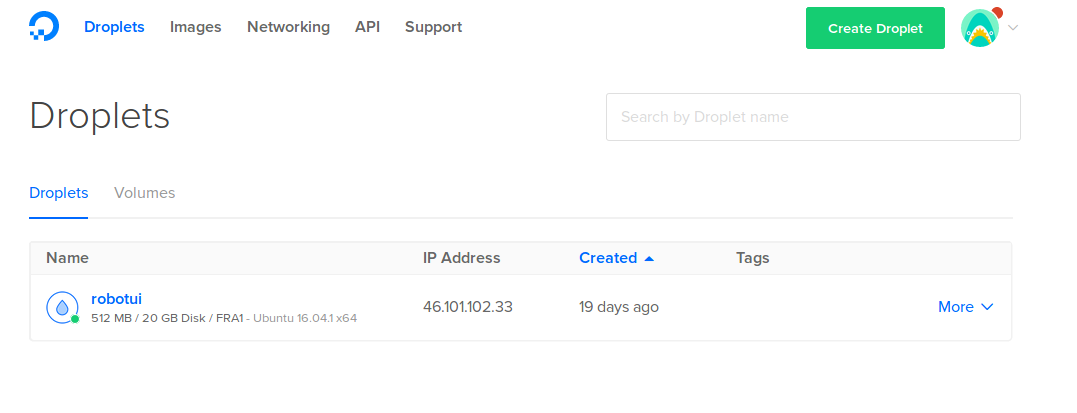
\includegraphics[scale=0.45]{imagenes/droplets.png}
\caption{Droplet desplegado en DigitalOcean}
\end{center}
\end{figure}


\subsection{Node js}

\begin{center}

\includegraphics[scale=0.3]{imagenes/nodejs-logo.png}
\end{center}

Web: \url{https://nodejs.org/es/}\\

Node.js es un entorno de ejecución para JavaScript construido con el motor de JavaScript V8 de Chrome. Node.js usa un modelo de operaciones E/S sin bloqueo y orientado a eventos, que lo hace liviano y eficiente. Incorpora un sistema de gestión de paquetes llamado, npm, es el ecosistema mas grande de librerías de código abierto en el mundo.\\

Node.js tiene una arquitectura basada en eventos capaz de E/S asíncronos. Estas opciones de diseño apuntan a optimizar el rendimiento y la escalabilidad en aplicaciones Web con muchas operaciones de entrada/salida, así como para aplicaciones Web en tiempo real (por ejemplo, programas de comunicación en tiempo real y juegos de navegador), lo que lo hacen ideal para este proyecto.\\


\subsection{Sails js}

\begin{center}

\includegraphics[scale=0.3]{imagenes/sailsjs-logo.png}
\end{center}

Web: \url{http://sailsjs.com/}\\

Sails.js es un framework web que facilita la creación de aplicaciones personalizadas Node.js de nivel empresarial. Está diseñado para parecerse a la arquitectura MVC de frameworks como Ruby on Rails, pero con soporte para el estilo de desarrollo de aplicaciones web más moderno y orientado a datos.\\

Utiliza Express para funciones como la gestión de peticiones HTTP y websockets. Su envoltorio intuitivo de websockets lo hace especialmente bueno para construir características en tiempo real como por ejemplo un Chat, por estas razones se ha considerado como el framework más adecuado hasta la fecha para la elaboración de este proyecto.


\subsection{Npm}

\begin{center}

\includegraphics[scale=0.5]{imagenes/npm-logo.png}
\end{center}

Web: \url{https://www.npmjs.com/}\\

npm es el manejador de paquetes por defecto para Node.js, un entorno de ejecución para JavaScript. Utilizado para la descarga de las librerías incorporadas al proyecto.


\subsection{SocketIO}

\begin{center}

\includegraphics[scale=0.3]{imagenes/socketio-logo.png}
\end{center}

Web: \url{https://socket.io/}\\

Socket.io es una librería que nos permite manejar eventos en tiempo real mediante una conexión TCP y todo ello en JavaScript desde un cliente.
Es realmente potente y podemos hacer todo tipo de aplicaciones en tiempo real. 


Socket.IO es una biblioteca de JavaScript para aplicaciones web en tiempo real. Permite la comunicación bidireccional en tiempo real entre clientes web y servidores. Consta de dos partes: una biblioteca del lado del cliente
que se ejecuta en el navegador y una biblioteca del lado del servidor para Node.js. Ambos componentes tienen una API casi idéntica. Al igual que Node.js, es impulsado por eventos.

Socket.IO puede usarse simplemente como un wrapper para WebSocket aunque proporciona muchas más funciones, incluyendo la transmisión a múltiples sockets, almacenamiento de datos asociados a cada cliente y E/S asíncronas.




\subsection{ FFmpeg }


\begin{center}

\includegraphics[scale=0.8]{imagenes/Ffmpeg-logo.jpg}
\end{center}

Web: \url{https://ffmpeg.org/}\\

FFmpeg es una colección de software libre que puede grabar, convertir (transcodificar) y hacer streaming de audio y vídeo. Incluye libavcodec, una biblioteca de códecs. FFmpeg está desarrollado en GNU/Linux, pero puede ser compilado
en la mayoría de los sistemas operativos, incluyendo Windows.

FFmpeg es un programa bastante sencillo y muy fácil de usar, orientado tanto a personas con conocimientos avanzados como usuarios inexpertos. 

El proyecto FFmpeg está compuesto por:

\begin{itemize}
 \item ffmpeg: es una herramienta de línea de comandos para convertir audio o video de un formato a otro. También puede capturar y codificar en tiempo real desde DirectShow, una tarjeta de televisión u otro dispositivo compatible.
 \item ffserver: es un servidor de streaming multimedia de emisiones en directo que soporta HTTP (la compatibilidad con RTSP está en desarrollo). Todavía no está en fase estable, y de momento no está disponible para Windows.
 \item ffplay: es un reproductor multimedia basado en SDL y las bibliotecas FFmpeg.
 \item libavcodec: es una biblioteca que contiene todos los códecs de FFmpeg. Muchos de ellos fueron desarrollados desde cero para asegurar una mayor eficiencia y un código altamente reutilizable.
 \item libavformat: es una biblioteca que contiene los multiplexadores/demultiplexadores para los archivos contenedores multimedia.
 \item libavutil: es una biblioteca de apoyo que contiene todas las rutinas comunes en las diferentes partes de FFmpeg.
 \item libpostproc: es una biblioteca de funciones de postproceso de vídeo.
 \item libswscale: es la biblioteca de escalado de vídeo.
\end{itemize}

Para el desarrollo de RobotUI, concretamente para la transmisión de vídeo desde el robot de pruebas desarrollado hacia el cliente, el módulo utilizado ha sido el de la herramienta de línea de comandos.


\subsection{Bootstrap}


\begin{center}

\includegraphics[scale=0.3]{imagenes/bootstrap-logo.jpg}
\end{center}

Web: \url{http://getbootstrap.com/}\\

Bootstrap es un framework o conjunto de herramientas de Código abierto para diseño de sitios y aplicaciones web. Contiene plantillas de diseño con tipografía, formularios, botones, cuadros, menús de navegación y otros elementos de diseño basado en HTML y CSS, así como, extensiones de JavaScript opcionales adicionales. Se ha utilizado en el presente proyecto para la maquetación de la aplicación.

\subsection{JQuery}


\begin{center}

\includegraphics[scale=0.6]{imagenes/jquery-logo.png}
\end{center}

Web: \url{https://jquery.com/}\\

JQuery es una biblioteca de JavaScript rápida, pequeña y característica. Hace que las cosas como HTML documento transversal y manipulación, manejo de eventos, animación, y Ajax mucho más simple con una fácil de usar API que funciona a través de una multitud de navegadores. Con una combinación de versatilidad y extensibilidad, jQuery ha cambiado la forma en que millones de personas escriben JavaScript.\\


\subsection{Mongo DB}

\begin{center}

\includegraphics[scale=0.5]{imagenes/mongodb-logo.png}
\end{center}


Web: \url{https://www.mongodb.com/es}\\

MongoDB (de la palabra en inglés “humongous” que significa enorme) es un sistema de base de datos NoSQL orientado a documentos, desarrollado bajo el concepto de código abierto.\\

MongoDB forma parte de la nueva familia de sistemas de base de datos NoSQL. En lugar de guardar los datos en tablas como se hace en las base de datos relacionales, MongoDB guarda estructuras de datos en documentos similares a JSON con un esquema dinámico (MongoDB utiliza una especificación llamada BSON), haciendo que la integración de los datos en ciertas aplicaciones sea más fácil y rápida.\\



\subsection{Pm2}

\begin{center}
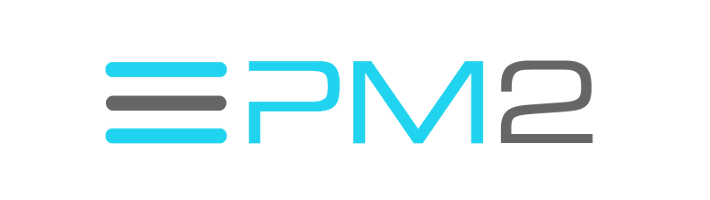
\includegraphics[scale=0.5]{imagenes/pm2-logo.png}
\end{center}

Web: \url{http://pm2.keymetrics.io/}\\


PM2 es un gestor de procesos de producción para aplicaciones Node.js con un equilibrador de carga incorporado. Le permite mantener las aplicaciones vivas para siempre, recargarlas sin tiempo de inactividad
y facilitar las tareas comunes del administrador del sistema.


\subsection{ Robomongo }

\begin{center}

\includegraphics[scale=0.5]{imagenes/robomongo-logo.png}
\end{center}

Web: \url{https://robomongo.org/}\\


Robomongo es una herramienta de gestión MongoDB de código abierto multi-plataforma basada en shell que incorpora el mismo motor de JavaScript que potencia el shell mongo de MongoDB.
Robomongo no sólo analiza la semántica del código, sino que también lo ejecuta en una máquina virtual JavaScript interna, lo que nos permite darle un autocompletado en tiempo de ejecución, 
imposible de obtener de forma estática. Siendo de especial ayuda para la gestión de la base de datos del proyecto.\\


\section{Tecnologías hardware y materiales utilizados}
\sectionmark{Tecnologías hardware}
\label{sec:tecnologias-hardware}



\subsection{Raspberry Pi Model B}
\label{sec:raspberry}

\begin{figure}[H]
  \begin{center}
    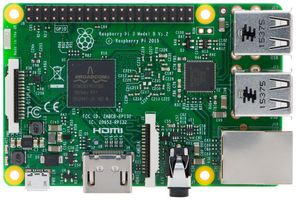
\includegraphics[scale=0.5]{imagenes/raspberry-pi.jpg}\\
    \caption{Imagen de una Raspberry Pi 3 Model B}
  \end{center}
\end{figure}

Web: \url{https://www.raspberrypi.org}\\


La Raspberry Pi 3 es la tercera generación de Raspberry Pi. Sus especificaciones son las siguientes:

\begin{itemize}
 \item Una CPU ARMv8 quad-core de 64 bits de 64 bits y 1.2 GHz
 \item LAN inalámbrica 802.11n
 \item Bluetooth 4.1
 \item Bluetooth baja energía (BLE)
 \item 1 GB de RAM
 \item 4 puertos USB
 \item 40 conexiones GPIO
 \item Puerto HDMI
 \item Puerto Ethernet
 \item Conector de audio combinado de 3,5 mm y vídeo compuesto
 \item Interfaz de la cámara (CSI)
 \item Interfaz de pantalla (DSI)
 \item Ranura para tarjeta Micro SD
 \item VideoCore IV núcleo de gráficos 3D 
\end{itemize}


\subsection{Controladora de motores L298N}


El módulo controlador de motores L298N H-bridge nos permite controlar la velocidad y la dirección de dos motores de corriente continua o un motor paso a paso de una forma muy sencilla,
gracias a los 2 los dos H-bridge que dispone.\\

básicamente un puente-H o H-bridge es un componente formado por 4 transistores que nos permite invertir el sentido de la corriente, y de esta forma podemos 
invertir el sentido de giro del motor.\\

El rango de tensiones en el que trabaja este módulo va desde 3V hasta 35V, y una intensidad de hasta 2A. A la hora de alimentarlo hay que tener en cuenta que la 
electrónica del módulo consume unos 3V, así que los motores reciben 3V menos que la tensión con la que alimentemos el módulo.\\

Además el L298N incluye un regulador de tensión que nos permite obtener del módulo una tensión de 5V, perfecta para alimentar nuestro Arduino. Eso sí, este regulador sólo 
funciona si alimentamos el módulo con una tensión máxima de 12V.\\

Es un módulo que se utiliza mucho en proyectos de robótica, por su facilidad de uso y su reducido precio.

\begin{figure}[H]
  \begin{center}
    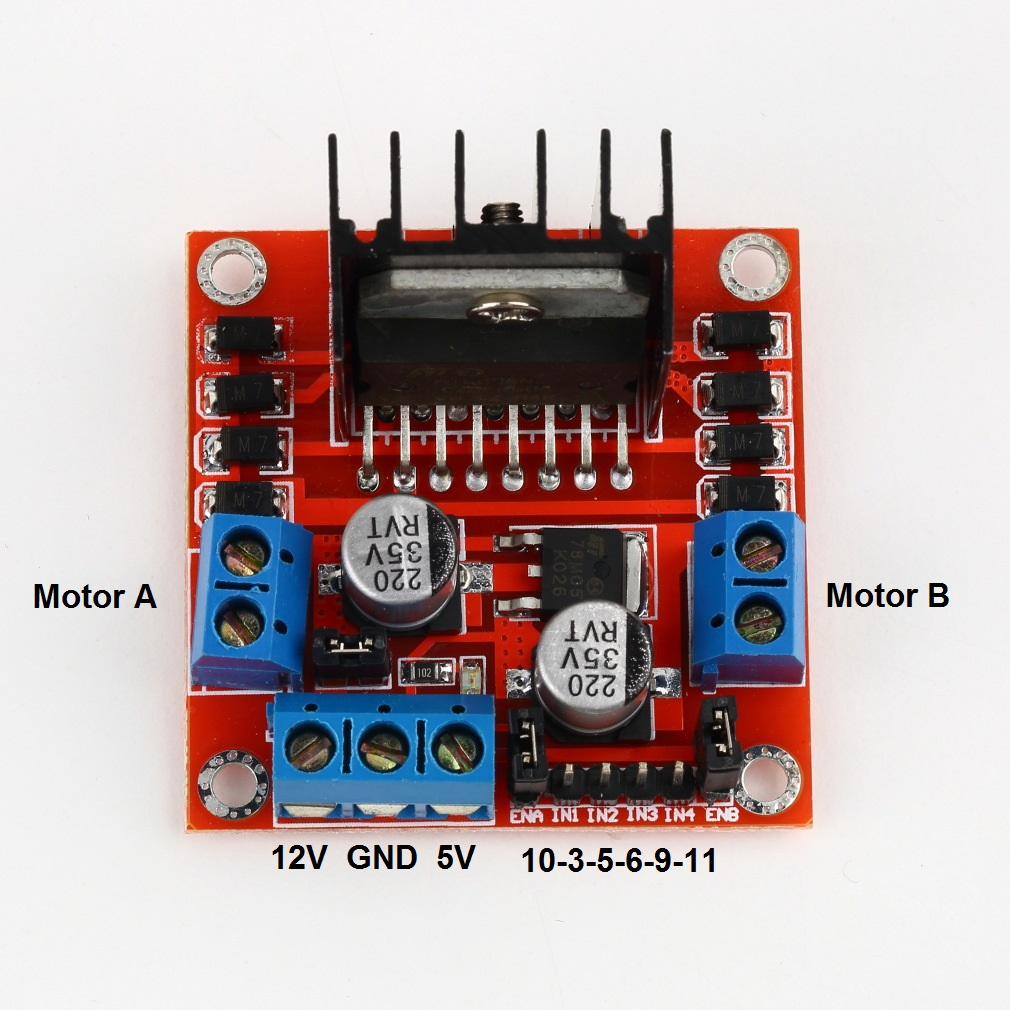
\includegraphics[scale=0.8]{imagenes/l298n.jpg}\\
    \caption{Imagen de la controladora de motores L298n utilizada}
  \end{center}
\end{figure}



\subsection{ Batería LiPo }

Para alimentar los motores y su controladora se ha empleado una batería LiPo de 1000mAh a 3,7V. Las batería de polímero de iones de litio, son pilas recargables (células de secundaria), compuestas generalmente de varias células secundarias idénticas en paralelo para aumentar la capacidad 
de la corriente de descarga. Siendo ideales para este tipo de usos.

\begin{figure}[H]
  \begin{center}
    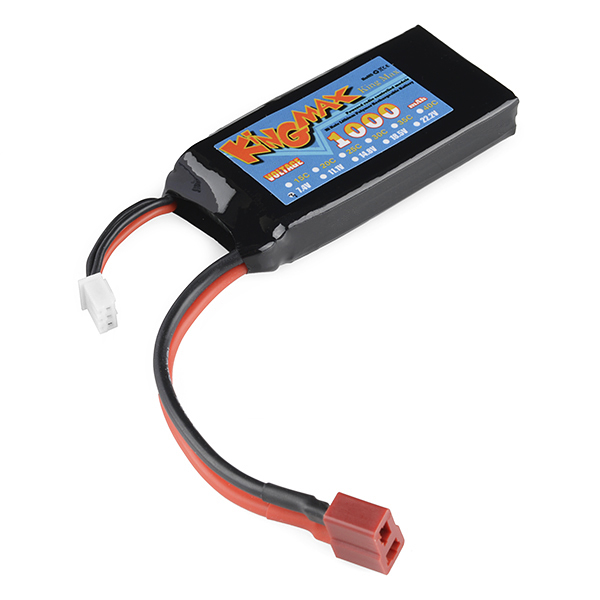
\includegraphics[scale=0.3]{imagenes/robot/bateria-lipo.jpg}\\
    \caption{Imagen de la batería LiPo utilizada.}
  \end{center}
\end{figure}


\subsection{ Tarjeta de expansión con batería de Litio para Raspberry Pi }
\label{componente:bateria-expansion}

Para la alimentación de la placa se ha optado por un módulo de potencia diseñado especialmente para la Raspberry Pi 3 Model B, permitiendo que la placa maestra trabaje sin conexión hasta 9 horas
de forma ininterrumpida.\\

Por otra parte, esta placa dispone de 2 puertos USB adicionales: uno suministra energía para la Raspberry Pi y el otro para una posible pantalla LCD, resultlando interesante para otros proyectos.\\

Sus características principales son las siguientes:

\begin{enumerate}
 \item Capacidad de la batería: 3800mAH
 \item Corriente de descarga máxima: 1.8A
 \item Tensión de salida sin carga: 5.1V ± 0.1V
 \item Corriente / voltaje de carga estándar: 1.0A / 5.0V
 \item Tensión de corte de la carga completa de la batería de iones de litio: 4.18V - 4.2V
\end{enumerate}


\begin{figure}[H]
  \begin{center}
    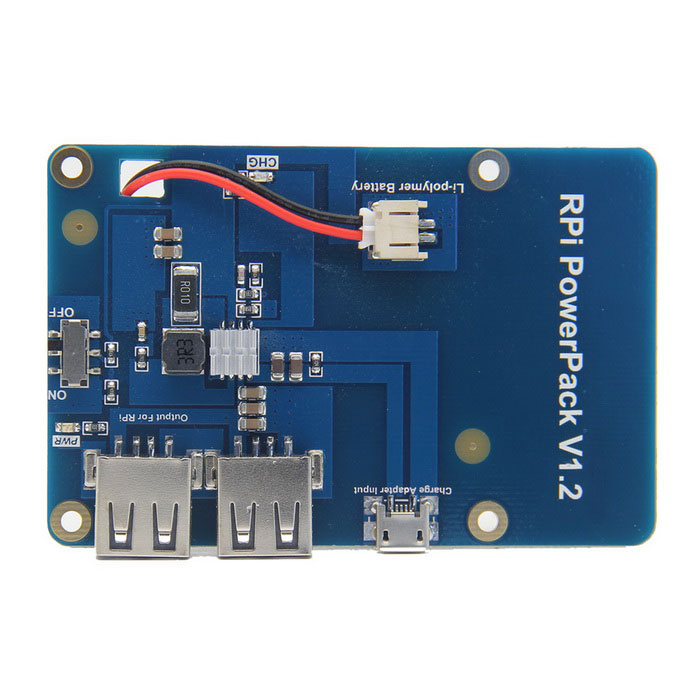
\includegraphics[scale=0.3]{imagenes/robot/modulo-alimentacion.jpg}\\
    \caption{Imagen de la tarjeta de expansión con batería de Litio utilizado.}
  \end{center}
\end{figure}

\subsection{ Cámara USB de alta definición }

Cámara USB para su conexión en la Raspberry para la emisión de imágenes. La cámara seleccionada dispone de las siguientes características:

\begin{itemize}
\item 2 megapíxeles de resolución.
\item Ángulo de visión de 170 grados.
\item Interfaz USB 2.0 de alta velocidad, refresco de 60 fps en resolución 1280X720, 30 fps en resolución 1920X1080
\item Tamaño reducido y perfil delgado ideal para aplicaciones embebidas.
\end{itemize}

\begin{figure}[H]
  \begin{center}
    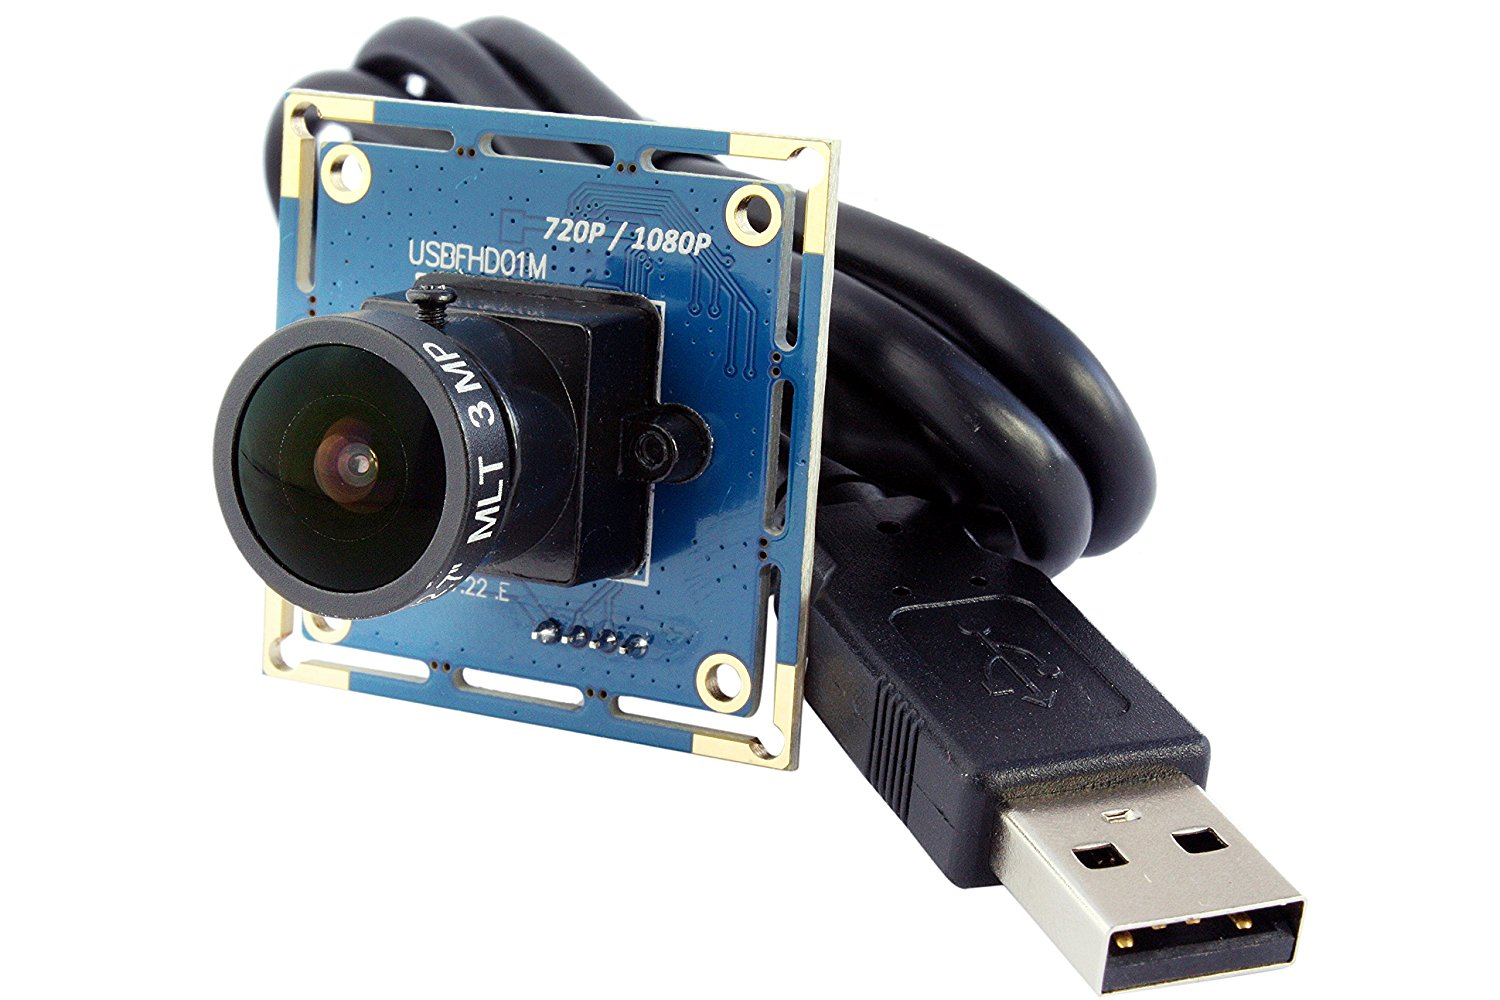
\includegraphics[scale=0.15]{imagenes/robot/camara-usb.jpg}\\
    \caption{Imagen de la cámara USB utilizada.}
  \end{center}
\end{figure}
